% ------------------------------------------------
\StartChapter{Methodology}{chapter:methodology}
% ------------------------------------------------
This section provides a detailed outline of our methodology. Initially, we discuss Discourse Coherence Learning, which employs a dialogue-enhanced graph encoder, detailed further in Section 3.2. Subsequently, we explore Persona Consistency Learning, where we examine the relationship between persona descriptions and dialogue, as covered in Section 3.3. Finally, we describe our Personalized Response Generation process, which integrates information from the aforementioned steps, elaborated in Section 3.4.

\begin{figure}[ht]
    \centering
    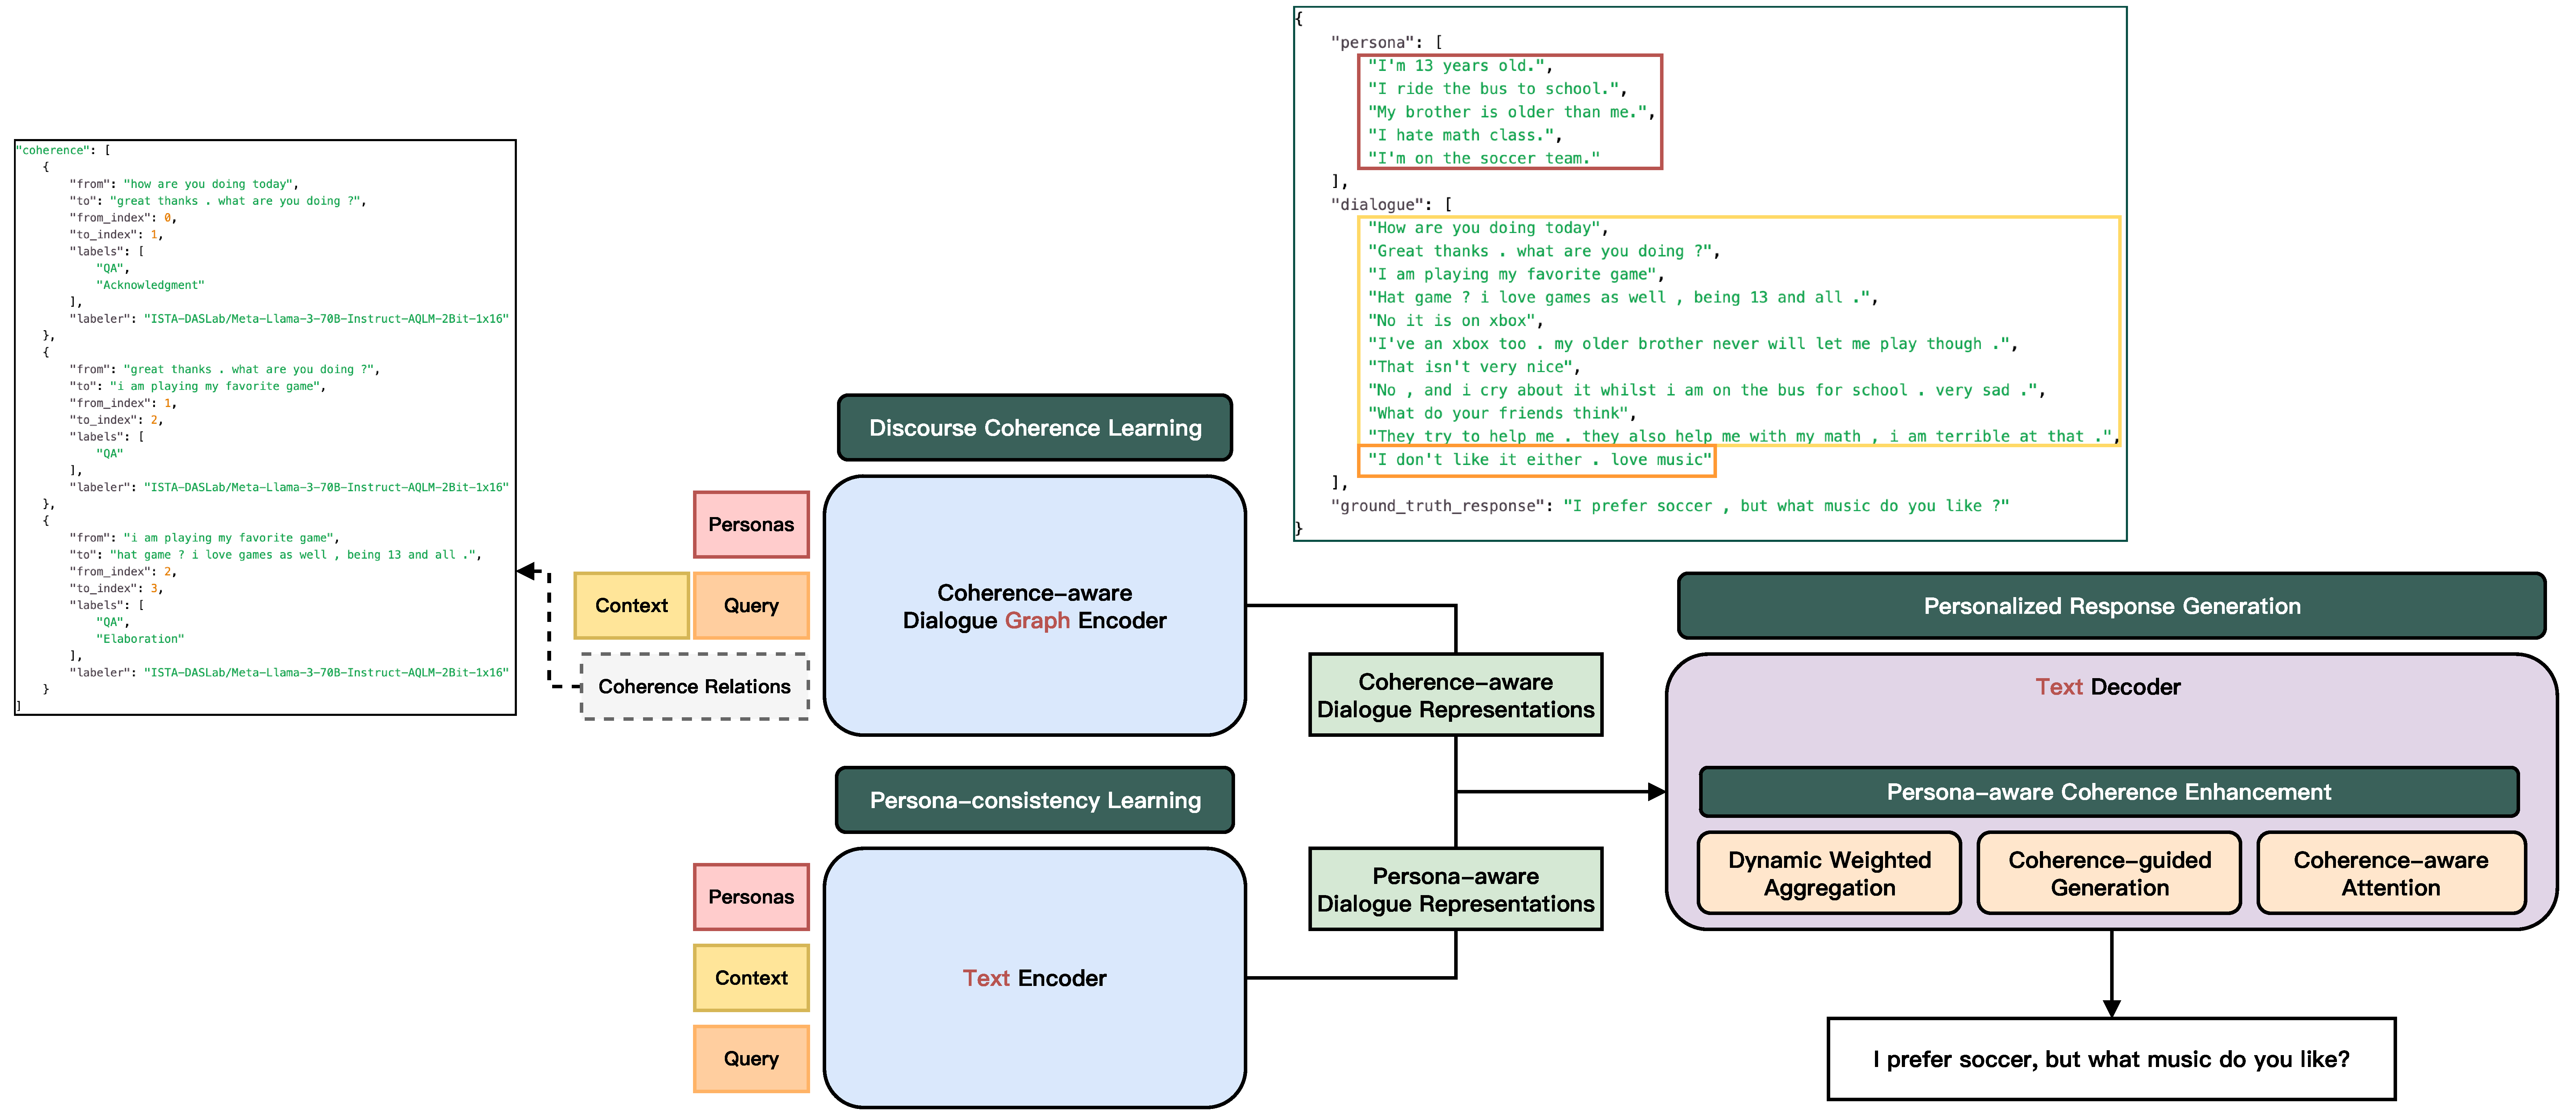
\includegraphics[width=1.00\textwidth]{./context/methodology/images/methodology_arch-v2.pdf}
    \caption{The overview framework of our method.}
    \label{fig:proposed_method_overview}
\end{figure}

Our method, depicted in Figure \ref{fig:proposed_method_overview}, accomplishes effective personalized dialogue generation via three key steps:

\begin{enumerate}
    \item \textbf{Discourse Coherence Learning:} We utilize a dialogue-enhanced graph encoder to model and understand the coherence of conversations, ensuring that the generated responses maintain logical continuity both locally and globally.

    \item \textbf{Persona-Consistency Learning:} This step involves analyzing and learning the intricate relationship between the persona information and the dialogue content to ensure that responses are not only relevant but also accurately reflect the traits of the persona.

    \item \textbf{Personalized Response Generation:} By integrating information from previous steps, this process customizes each response to reflect the discourse relations, context, and persona via our proposed mechanisms, thereby improving the conversation's coherence and personalization.
\end{enumerate}

Figure \ref{fig:proposed_model_arch} illustrates the overall architecture of our model, termed \textbf{MUDI (Multiple Discourse Relations Graph Learning)}, which enhances persona-consistent dialogue generation. The backbone of \textbf{MUDI} is based on GATv2 \cite{brody-etal-2022-gatv2} and BART \cite{lewis-etal-2020-bart}.

\begin{figure}[ht]
    \centering
    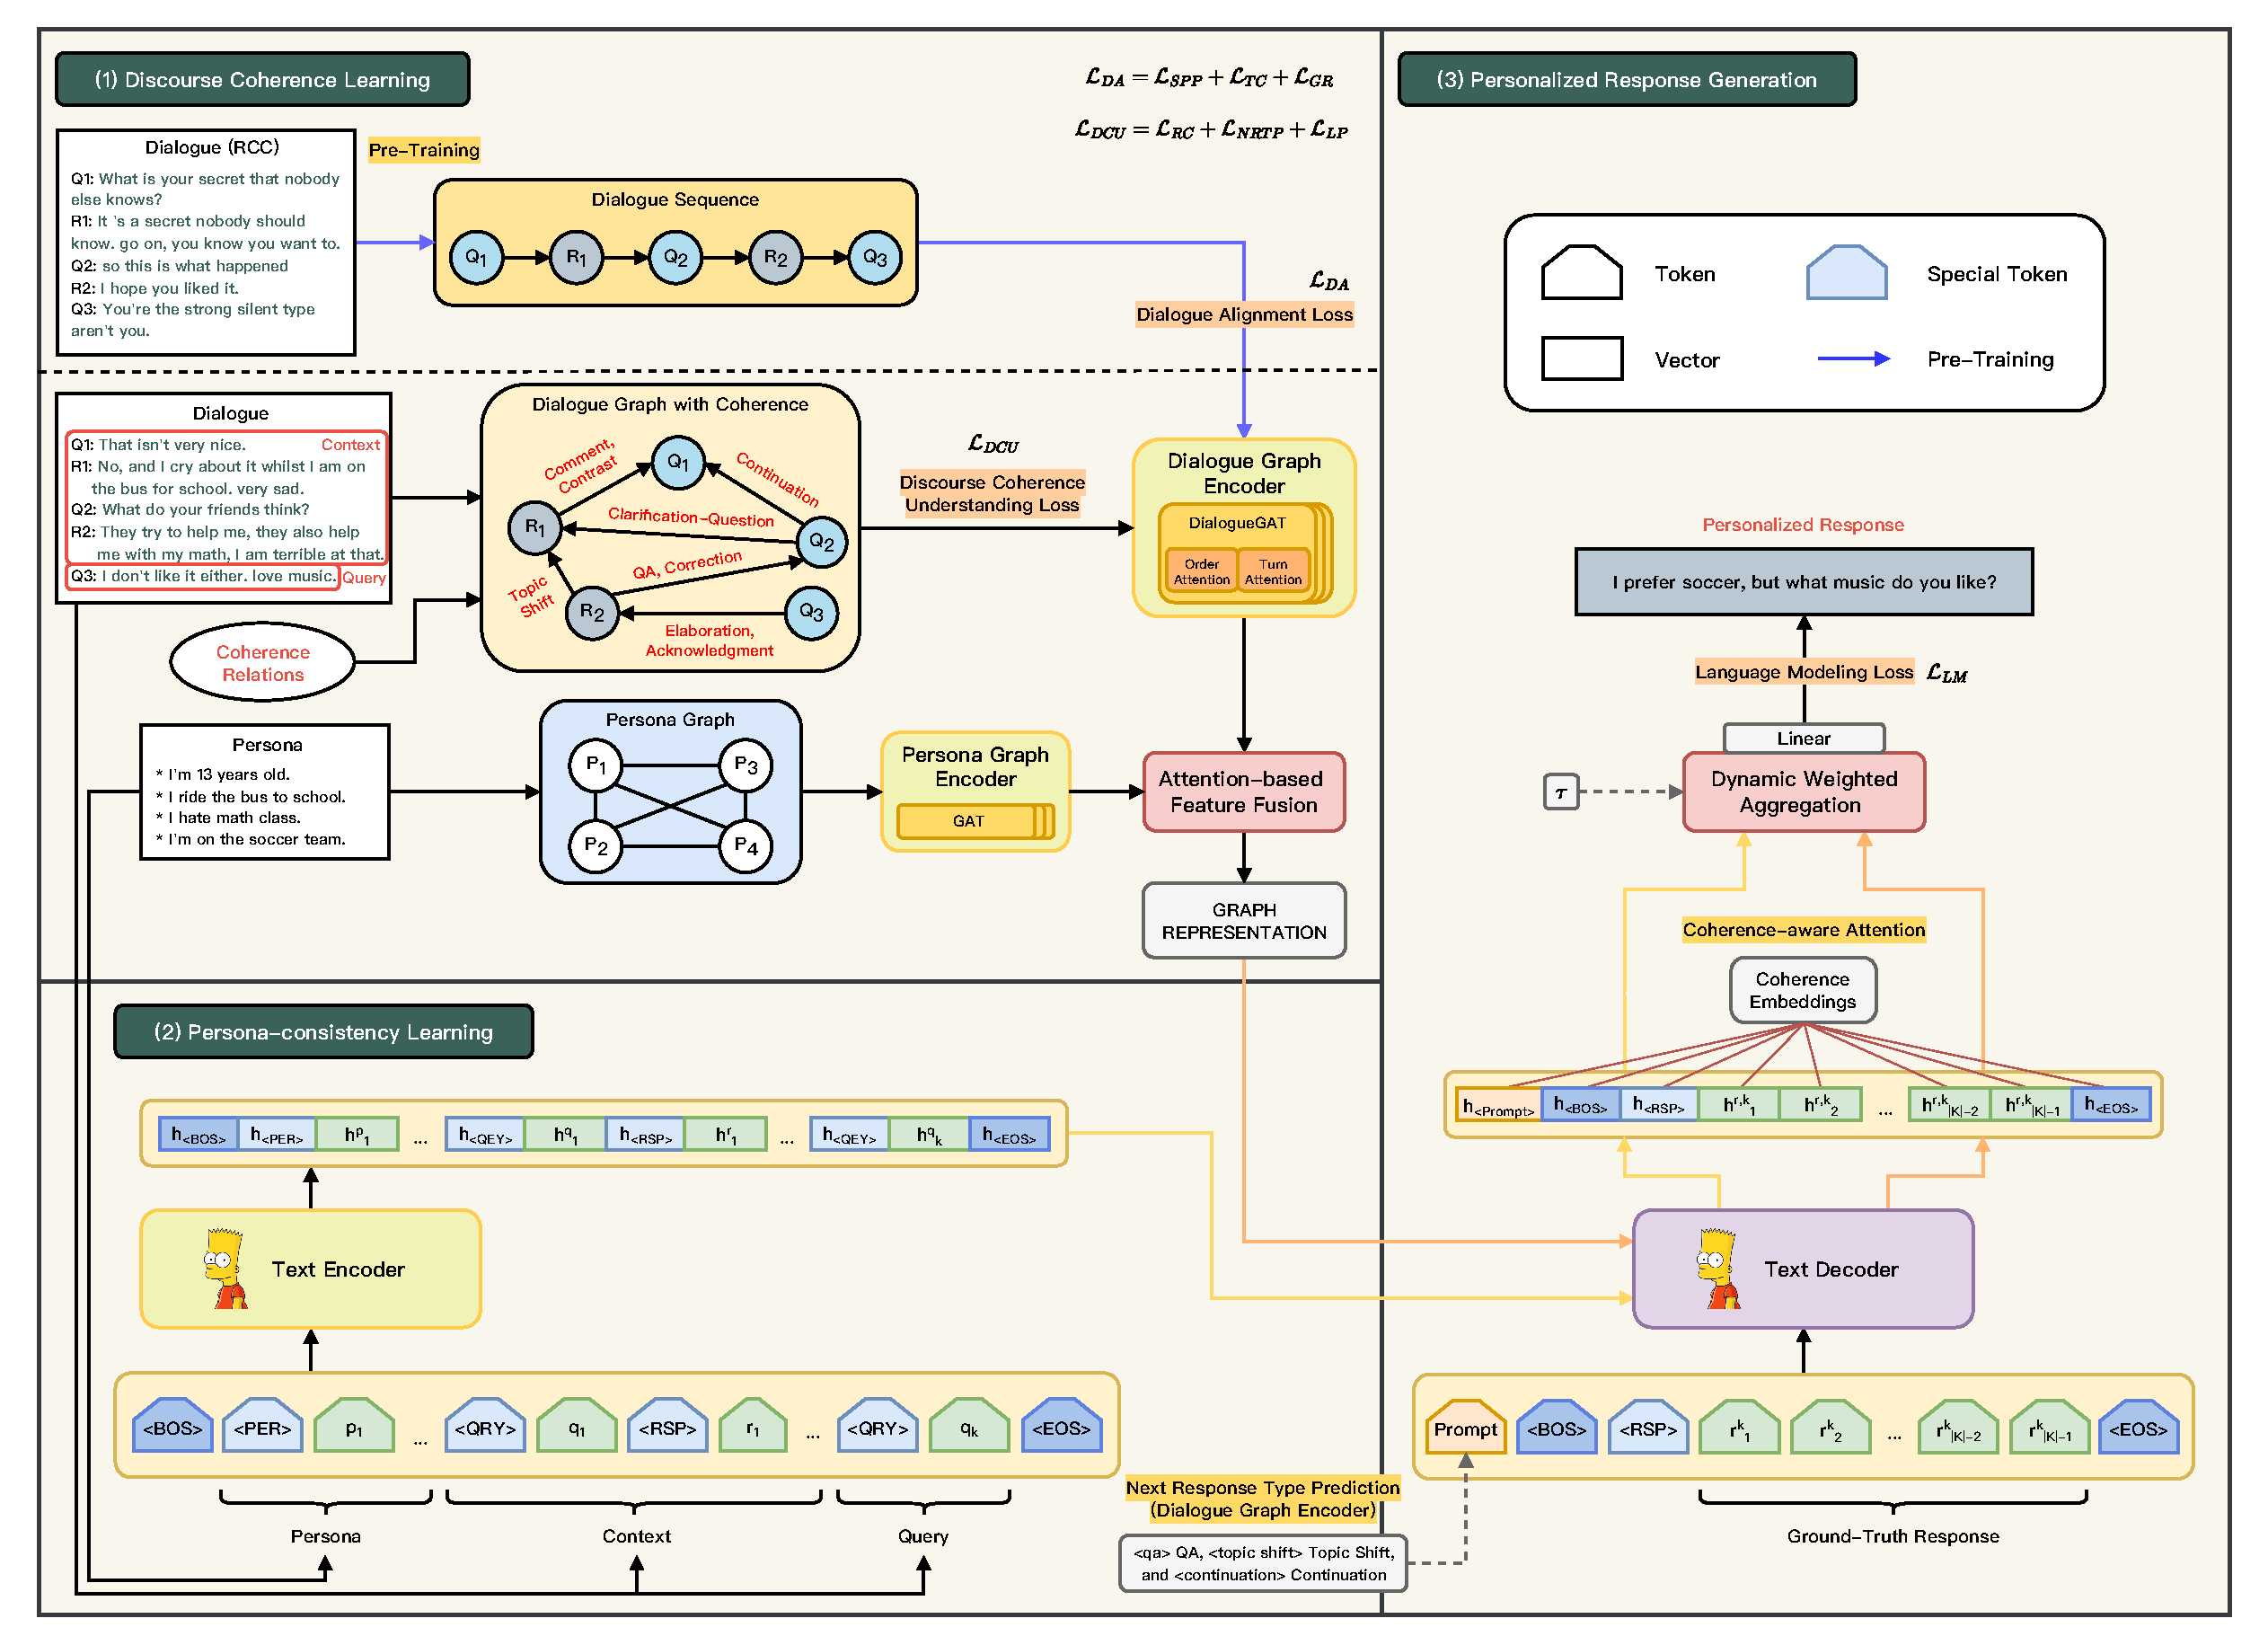
\includegraphics[width=1.05\textwidth]{./context/methodology/images/research_model_arch-v5.pdf}
    \caption{The overall architecture of our model - MUDI.}
    \label{fig:proposed_model_arch}
\end{figure}

\section{Problem Definition}
The task involves generating a personalized response, denoted as $r_{|K|}$, given the persona descriptions $P = \{p_{1}, p_{2}, ... , p_{|\text{P}|}\}$ and a multi-turn dialogue context $C = \{q_{1}, r_{1}, q_{2}, r_{2}, ... ,\\ q_{|\text{\text{K}}|−1}, r_{|\text{K}|−1}, q_{|\text{K}|}\}$. In this context, $q$ and $r$ represent the user query and the chatbot response, respectively. The core goal of personalized response generation is to accurately estimate the probability distribution $p(r | C, P)$, facilitating the generation of specifically tailored responses that reflect the persona information and dialogue history.

\textbf{Enhancing Coherence:}  An ideal personalized response should be not only natural but also consistent with the persona. To generate a more coherent response, we incorporate the discourse relations outlined in Section 3.2.1. With specific response types $T = \{t_{1}, t_{2}, ... , t_{|T|}\}$ identified, our goal extends to producing a response $r_{|K|}$ that seamlessly integrates these types across the dialogue. Consequently, we aim to optimize the probability $p(r | C, P, T)$, enhancing both the personalization and coherence of the responses generated.

\section{Discourse Coherence Learning}
\label{sec:discourse_coherene_learning}
Our method leverages discourse relations to enhance the coherence of dialogue generation. We employ a Graph Neural Network (GNN) model specifically designed to learn these relations. To further improve the GNN's ability to understand dialogue structure, we have enhanced the existing model by incorporating a mechanism to capture dialogue structure. Additionally, we adopt a pretrain-finetune strategy to optimize performance. The detailed description of these enhancements is as follows.

\subsection{Coherence Relations Annotation} \label{sec:coherence_reltaions_annotation}
To facilitate the model's understanding of how two sentences in a conversation are effectively connected, we employ Large Language Models (LLMs) such as GPT-4, Mixtral-8x7b, and LLaMA-3 to assist in annotating coherence relations. There are, in total, 16 discourse relations according to STAC \cite{asher-etal-2016-discourse}, namely, \textbf{comment}, \textbf{clarification-question}, \textbf{elaboration}, \textbf{acknowledgment}, \textbf{continuation}, \textbf{explanation}, \textbf{conditional}, \textbf{question-answer}, \textbf{alternation}, \textbf{question-elaboration}, \textbf{result}, \textbf{background}, \textbf{narration}, \textbf{correction}, \textbf{parallel} and \textbf{contrast}. On top of these relationships, we add \textbf{topic-shift} to represent coherent topic transitions between conversations. 

Each pair of utterances could be annotated with zero to three different relations. In total, we have annotated 1,942,177 pairs of utterances for their coherence relations. An example of annotated results can be seen in Table \ref{table:coherence-relations-annotated-example}. The prompt for coherence relations annotations is shown in Figure \ref{fig:coherence_reltaions_annotated_prompt}

\begin{table}[H]
\centering
\def\arraystretch{1.4}%
\begin{tabular}{|c|l|c|}
\hline

\rowcolor[RGB]{204,217,245}
\textbf{Index} & \multicolumn{2}{|c|}{\textbf{Dialogue}} \\
\hline

0 & \multicolumn{2}{|p{14cm}|}{[PERSON 1:] Hello what are doing today?} \\
\cline{1-1}
1 & \multicolumn{2}{|p{14cm}|}{[PERSON 2:] I am good, I just got off work and tired, I have two jobs.} \\
\cline{1-1}
2 & \multicolumn{2}{|p{14cm}|}{[PERSON 1:] I just got done watching a horror movie.} \\
\cline{1-1}
3 & \multicolumn{2}{|p{14cm}|}{[PERSON 2:] Wow! I do love a good horror movie. Loving this cooler weather.} \\
\cline{1-1}
4 & \multicolumn{2}{|p{14cm}|}{[PERSON 1:] But a good movie is always good.} \\
\cline{1-1}
5 & \multicolumn{2}{|p{14cm}|}{...} \\
\hline

\rowcolor[RGB]{204,217,245}
\textbf{Index} & \multicolumn{1}{|c|}{\textbf{Utterance}} & \textbf{Coherence Relations} \\
\hline

0 & Hello what are doing today? & \multirow{2}{*}{QA, Explanation} \\
\cline{1-2}
1 & I am good, I just got off work and tired, I have two jobs. & \\
\hline

0 & Hello what are doing today? & \multirow{2}{*}{QA} \\
\cline{1-2}
2 & I just got done watching a horror movie. & \\

\hline
\multicolumn{3}{|c|}{...} \\
\hline

1 & I am good, I just got off work and tired, I have two jobs. & \multirow{2}{*}{Topic Shift} \\
\cline{1-2}
2 & I just got done watching a horror movie. & \\
\hline

\multicolumn{3}{|c|}{...} \\
\hline

\end{tabular}
\caption{Examples of coherence relations annotated by the LLaMA-3-70B\protect\footnotemark\cite{llama3modelcard}. We annotated all utterance pairs in the dialogue, and the examples shown here represent only a subset of the complete dataset.}
\label{table:coherence-relations-annotated-example}
\end{table}
\footnotetext{https://huggingface.co/meta-llama/Meta-Llama-3-70B-Instruct}

\InsertFigure
[scale=0.18,
caption={The prompt of Coherence Relations Annotation.},
label={fig:coherence_reltaions_annotated_prompt}
]
{./context/methodology/images/coherence_reltaions_annotated_prompt.png}

\subsection{Dialogue Graph Modeling}
To enable the model to capture discourse coherence information within conversations when generating responses, and inspired by the success of previous graph-based discourse modeling efforts \cite{dong-etal-2021-discourse}, \cite{feng-etal-2021-dialogue}, \cite{li-etal-2021-dadgraph}, we employ a Graph Neural Network (GNN) as the dialogue encoder to learn the interactive relationships between discourses. To account for sentence-level semantics, we utilize the Sentence-Transformer \cite{reimers-2019-sentence-bert} as an encoder to extract contextualized global semantics from both utterances and personas, thereby initializing the node features.

In our method, we found that the powerful GNN models that have been proposed, such as GCN, GAT, GraphSAGE, etc., are not specifically designed for dialogue structure and may not fully capture the intricate structure and complex long-term interactions in conversations. To overcome this, we enhance the GATv2 \cite{brody-etal-2022-gatv2} model by incorporating structures that specifically capture dialogue information. Specifically, We introduce two key modifications to capture the dialogue structure: Order information and Turn information, both integrated via an attention mechanism. We call this dialogue-enhanced GNN is \textbf{DialogueGAT}. The Example of Order-Attention and Turn-Attention as illustrated in Figure \ref{fig:dialoguegat}. The specific introduction to these two mechanisms is as follows:

\subsubsection{Order-Attention}
To model the sequential nature of dialogues, we introduce auxiliary edges connecting each utterance to its $k{\text -}hop$ neighboring utterances based on their order. This indicator could formalized as Eq. \ref{eq:add_order_auxiliary_edges}. Then $d=k+1$, where $d$ represents the difference.

\begin{equation}\label{eq:add_order_auxiliary_edges}
    I(i, j, d) = 
    \begin{cases} 
    1 & \text{if } \operatorname{order}(j) > \operatorname{order}(i) \text{ and } |\operatorname{order}(i) - \operatorname{order}(j)| < d \\
    0 & \text{otherwise}
    \end{cases}
\end{equation}

The attention scores between nodes are calculated based on the exponential decay of the order difference, as described in Eq. \ref{eq:dialoguegat_order_exp_decay}, \ref{eq:dialoguegat_order_act}, \ref{eq:dialoguegat_attn}, and \ref{eq:dialoguegat_hidden_states}. Here, $\lambda$ represents the decay rate.

\begin{equation}\label{eq:dialoguegat_order_exp_decay}
    s_{ij} = \exp(-\lambda \cdot |\operatorname{order}(i) - \operatorname{order}(j)|) \cdot I(i, j, d)
\end{equation}

\begin{equation}\label{eq:dialoguegat_order_act}
    e(h_i, h_j) = (\alpha^T \cdot \text{LeakyReLU}(W \cdot [h_i \parallel h_j])) \cdot s_{ij}
\end{equation}

\begin{equation}\label{eq:dialoguegat_attn}
    \alpha_{ij} = \text{softmax}_j \left( e(h_i, h_j) \right) = \frac{\exp(e(h_i, h_j))}
    {\sum_{j' \in N_i} \exp(e(h_i, h_{j'}))}
\end{equation}

\begin{equation}\label{eq:dialoguegat_hidden_states}
    h_i' = \sigma \left( \sum_{j \in N_i} \alpha_{ij} \cdot W h_j \right)
\end{equation}

\subsubsection{Turn-Attention}
We also incorporate turn information by adding bidirectional auxiliary edges between utterance nodes within the same turn, as described in Eq. \ref{eq:add_turn_auxiliary_edges}

\begin{equation}\label{eq:add_turn_auxiliary_edges}
    t_{ij} = 
    \begin{cases} 
    1 & \text{if } \text{turn}(i) = \text{turn}(j) \\
    0 & \text{otherwise}
    \end{cases}
\end{equation}

Then, we calculate the attention scores between nodes of the same conversational turn in the same manner. These calculations are detailed in Eq. \ref{eq:dialoguegat_turn_act}, \ref{eq:dialoguegat_attn}, and \ref{eq:dialoguegat_hidden_states}.

\begin{equation}\label{eq:dialoguegat_turn_act}
    e(h_i, h_j) = (\alpha^T \cdot \text{LeakyReLU}(W \cdot [h_i \parallel h_j])) \cdot t_{ij}
\end{equation}

\InsertFigure
[scale=0.17,
caption={The visualizations of Order-connection and Turn-connection in our proposed DialogueGAT model. Illustrates how the red connections denote turn information and the purple connections indicate order information, with $k = 2$ for order connections.},
label={fig:dialoguegat}
]
{./context/methodology/images/dialoguegat.png}

\subsubsection{Pre-training Phase}
During the pre-training phase, our objective is to enhance the Graph encoder's ability to comprehend and capture the structure of dialogue data effectively. To achieve this, we perform pre-training on the large-scale dialogue dataset Reddit Conversation Corpus (5-turns) \cite{dziri-etal-2019-augmenting}. Drawing inspiration from the strategies outlined in \cite{wu-etal-2023-gnn-pretrain}, we have designed three specific self-supervised pretraining tasks to aid the model in understanding the intricate dialogue structure. These tasks include Shortest Path Prediction (SPP), which helps the model infer the most direct connections within dialogue sequences; Turn Classification (TC), which assists in recognizing the speaker's changes and continuities; and Graph Reconstruction (GR), aimed at enabling the model to rebuild dialogue sequences from scattered data points. Initially, we convert the raw dialogue data into structured dialogue sequences, and we employ a Graph Encoder to extract hidden states from the dialogue sequence. These hidden states are then utilized in three specific tasks, each with its own loss calculation:

\begin{equation}\label{eq:gnn_pre_enc}
    H = \text{GNN}_{\theta}(X^{\text{pre}},A^{\text{pre}})
\end{equation}
\begin{equation}\label{eq:gnn_pre_concat}
    h_{ij} = [H_i \parallel H_j]
\end{equation}

\begin{itemize}
    \item \textbf{Shortest Path Prediction}: This task involves predicting the shortest paths between sampled pairs of nodes from multiple dialogue graphs within a batch. Nodes are sampled across different graphs, and the model first concatenates the hidden states of the sampled nodes to form an input vector for the MLP. The predicted shortest path length between a sampled pair of nodes \(i\) and \(j\) is given by Eq. \ref{eq:gnn_pre_concat} \ref{eq:gnn_pre_spp_mlp}.
    \begin{equation}\label{eq:gnn_pre_spp_mlp}
        \hat{y}_{ij}^{\text{SPP}} = \text{MLP}(h_{ij})        
    \end{equation}
    The loss for this task, denoted as \( \mathcal{L}_{\text{SPP}} \), is computed using the mean squared error (MSE) over the sampled node pairs within the batch:
    \begin{equation}
        \mathcal{L}_{\text{SPP}} = \sum_{(i, j) \in S} (y_{ij}^{\text{SPP}} - \hat{y}_{ij}^{\text{SPP}})^2
    \end{equation}
    Where \( S \) is the set of sampled node pairs from the batch. If the sampled nodes \(i\) and \(j\) belong to different graphs, the ground truth shortest path length \( y_{ij}^{\text{SPP}} \) is assumed to be 0, reflecting the absence of a path between graphs.

    \item \textbf{Turn Classification}: This task involves classifying whether two sampled nodes within a batch correspond to utterances that occur in the same turn of a conversation. The model concatenates the hidden states of the sampled nodes to form an input vector for the MLP (Eq. \ref{eq:gnn_pre_concat} \ref{eq:gnn_pre_tc_mlp}), which predicts the probability that the two utterances belong to the same turn:
    \begin{equation} \label{eq:gnn_pre_tc_mlp}
        \hat{y}_{ij}^{\text{TC}} = \text{MLP}(h_{ij})
    \end{equation}
    The loss for this task, denoted as \( \mathcal{L}_{\text{TC}} \), is calculated using binary cross-entropy:
    \begin{equation}
        \mathcal{L}_{\text{TC}} = -\sum_{(i, j) \in S} \left( y_{ij}^{\text{TC}} \log(\hat{y}_{ij}^{\text{TC}}) + (1 - y_{ij}^{\text{TC}}) \log(1 - \hat{y}_{ij}^{\text{TC}}) \right)
    \end{equation}
    Where \( S \) is the set of sampled node pairs from the batch, \( y_{ij}^{\text{TC}} \) represents the ground truth label indicating whether the utterances of nodes \( v_i \) and \( v_j \) belong to the same turn, and \( \hat{y}_{ij}^{\text{TC}} \) is the predicted probability. Optimizing this turn classification loss helps to enhance the graph encoder's ability to identify directly related utterances within the dialogue.

    \item \textbf{Graph Reconstruction}: The objective of this task is to reconstruct the adjacency matrix of the dialogue graph using a method inspired by the Variational Graph Auto-Encoders (VGAE) described in Kipf et al. \cite{kipf-etal-2016-vgae}. We employ an inner product decoder to estimate the adjacency matrix from the hidden representations of the nodes. This approach calculates the probability of an edge existing between any two nodes based on their hidden states:
    \begin{equation}\label{eq:vgae_inner_product}
        p(A | H) = \prod_{i=1}^{N} \prod_{j=1}^{N} p(A_{ij} | h_i, h_j), \text{ with } p(A_{ij} = 1 | h_i, h_j) = \sigma(h_i^T h_j)
    \end{equation}
    where \( A_{ij} \) are the elements of the adjacency matrix \( A \), and \( \sigma(\cdot) \) is the logistic sigmoid function. The graph reconstruction loss, \( \mathcal{L}_{\text{GR}} \), is then calculated using binary cross-entropy:
    \begin{equation}
        \mathcal{L}_{\text{GR}} = -\sum_{i=1}^N \sum_{j=1}^N \left( A_{ij} \log(\sigma(h_i^T h_j)) + (1 - A_{ij}) \log(1 - \sigma(h_i^T h_j)) \right)
    \end{equation}
    This loss function quantifies the error in reconstructing the adjacency matrix, thereby guiding the model toward learning accurate node embeddings that reflect the actual graph structure.

\end{itemize}

Consider the pretraining tasks and their respective losses, the total loss $\mathcal{L}_{\text{DA}}$ (Dialogue Alignment) is then given by the sum of these individual losses:
\begin{equation}
    \mathcal{L}_{\text{DA}} = \mathcal L_{\text{SPP}} + \mathcal L_{\text{TC}} + \mathcal L_{\text{GR}}
\end{equation}

\subsubsection{Fine-tuning Phase}
During the finetuning stage, we utilize a personalized dialogue dataset annotated with coherence relations to learn the discourse relations in dialogue. The dataset allows us to finetune the pretrained Graph Encoder $\text{GNN}_{\theta}$ using enhanced data that includes not only the node features $X_{C}^{ft}$ and adjacency matrix $A_{C}^{ft}$ but also coherence relations $R$. Specifically, the node features $X_{C}^{ft}$ and adjacency matrix $A_{C}^{ft}$ are derived from the dialogue context $C$, where each node is connected to its $k{\text -}hop$ nearest neighbors to reflect the local conversational structure. This connectivity pattern helps in capturing the intricate dynamics of dialogue interactions. Due to the significant class imbalance in the labeled coherence relations, where some categories are overrepresented such as "Topic Shift", which may lead to the model excessively focusing on these categories during training, we address this issue by randomly pruning edges that are solely labeled with a high-frequency category. We refer to this graph as the "Dialogue Graph", and its specific visual representation can be seen in the yellow graph on the upper left of Figure \ref{fig:proposed_model_arch}.

This approach helps in balancing the distribution of classes and refining the model's understanding of diverse conversational patterns. The finetuning process updates the encoder to $\text{GNN}_{\theta'}$, adapting it more closely to the specificities of the personalized dialogues:
\begin{equation}\label{eq:gnn_ft_enc}
    H_{\text{C}} = \text{GNN}_{\theta'}(X_{C}^{\text{ft}}, A_{C}^{\text{ft}}, R)
\end{equation}

In addition, we transform persona sentences from the dialogue into a completed graph. This transformation enables the leveraging of a GAT \cite{brody-etal-2022-gatv2}, denoted as $\text{GNN}_{\psi}$, to better capture the nuances and importance of each persona sentence in relation to others. We refer to this graph as the "Persona Graph", and its specific visual representation can be seen in the blue graph on the upper left of Figure \ref{fig:proposed_model_arch}.
\begin{equation}
H_{\text{P}} = \text{GNN}_{\psi}(X_{P}, A_{P})
\end{equation}

Here, $X_{P}$ and $A_{P}$ represent the node features and adjacency matrix of the persona sentences, respectively. The graph encoder constructed from persona sentences applies its attention mechanism across all connections, enhancing the encoder's sensitivity to persona-specific information.

Next, we employ an attention-based feature fusion mechanism to integrate the utterance node representations of a specific speaker in the dialogue graph with the corresponding node representations in the persona graph. By using attention, the model can focus more on persona information that is relevant to this particular utterance. Specifically, we use a cross-attention approach where the persona information serves as the key and value, and the utterance information serves as the query. The feature fusion is then performed using a multi-head attention mechanism to obtain the personalized node representations, denoted as $H_{\text{D}}$:

\begin{equation}
\begin{aligned}
    H_{\text{D}} &= \text{MultiHead}(Q,K,V) = \text{Concat}(head_1, \ldots, head_h)W^O \\
    \text{where} \quad head_i &= \text{CrossAttention}(Q W^Q_i, K W^K_i, V W^V_i), \quad i = 1, \ldots, h \\
    Q &= H_{\text{C}} \cdot W^Q_i, \quad
    K = H_{\text{P}} \cdot W^K_i, \quad
    V = H_{\text{P}} \cdot W^V_i
\end{aligned}
\end{equation}

\begin{equation}
    \text{CrossAttention}(Q, K, V) = \text{softmax}\left(\frac{QK^T}{\sqrt{d_k}}\right)V
\end{equation}

Furthermore, we learn coherence relations through three tasks: Coherence Relations Classification (RC), Next Response Type Prediction (NRTP), and Link Prediction (LP).

\begin{itemize}
    \item \textbf{Coherence Relations Classification}: This task is a multi-label classification task. Given two nodes, the graph encoder predicts which of the 17 types of coherence relations defined in Section 3.2.1 exist between them. For each pair of nodes, the model outputs a set of labels indicating the applicable coherence relations. The model concatenates the hidden states of the nodes to form an input vector for the MLP (Eq. \ref{eq:gnn_ft_rc_mlp}), which predicts the probability of the relations between the two utterances:
    \begin{equation} \label{eq:gnn_ft_rc_mlp}
        \hat{y}_{ij}^{\text{RC}} = \text{MLP}([H_i \parallel H_j])
    \end{equation}
    The loss for this task, denoted as \( \mathcal{L}_{\text{RC}} \), is calculated using binary cross-entropy:
    \begin{equation}
        \mathcal{L}_{\text{RC}} = -\sum_{(i, j) \in E \subseteq A_{C}^{\text{ft}}} \left( y_{ij}^{\text{RC}} \log(\hat{y}_{ij}^{\text{RC}}) + (1 - y_{ij}^{\text{RC}}) \log(1 - \hat{y}_{ij}^{\text{RC}}) \right)
    \end{equation}
    Here, $E$ represents the edge set of connected node pairs within the same graph in the batch. \( y_{ij}^{\text{RC}} \) represents the ground truth labels indicating which of the 17 types of coherence relations exist between nodes $v_{i}$ and $v_j$, and \( \hat{y}_{ij}^{\text{RC}} \) is the predicted probability. In our implementation, we encountered a severe label imbalance problem in the coherence relations, exhibiting a long-tail distribution. For example, Topic Shift dominated most labels, leading to model prediction bias towards a few frequent categories. Therefore, we incorporated the Class-balance loss proposed by \cite{cui-etal-2019-cbloss}, which considers the weights between classes to mitigate the issue of the model being dominated by a minority of high-frequency labels. 
    
    Optimizing this coherence relations classification loss helps to enhance the graph encoder's ability to identify and distinguish different types of relations within the dialogue context.

    \item \textbf{Next Response Type Prediction}: This task aims to predict the possible types of the next response. This is also a multi-label classification task, where the model predicts which of the 17 types of coherence relations will be present in the next response. This task has two forms: The model predicts the kind of the next response based on the current utterance node, and the model predicts the type of the next response based on all previous utterances. Specifically, we first extract node representations from $H_D$ that have direct sequential relationships in the original dialogue to form a dialogue sequence $S$:

    \begin{equation}
    S = { h_{i_1}, h_{i_2}, \ldots, h_{i_t} } \quad \text{where} \quad h_{i_k} \in H_{D} \quad \text{and} \quad (i_k, i_{k+1}) \in E \subseteq A_{C}^{\text{ft}}
    \end{equation}
    
    Subsequently, we apply two methods to predict the response type:

    \begin{enumerate}
        \item Direct Prediction: For the first form, the model directly uses the hidden states of the current utterance node to predict the next response type.
        \begin{equation}
            \hat{y}_{i}^{\text{direct}} = \text{MLP}(\sigma(h_{i}))
        \end{equation}

        \item Sequential Prediction (auto-regressive style): For the second form, the model uses a sequential model, such as a GRU, to process the dialogue sequence \( S \) up to the \( (i-1) \)-th utterance.

        \begin{equation}
            \hat{y}_{i}^{\text{seq}} = \text{MLP}(\sigma(\text{GRU}(S_{1:i-1})))
        \end{equation}

        \end{enumerate}

    Both forms share the same MLP for the final prediction. The loss for this task, denoted as $\mathcal{L}{\text{NRTP}}^{\text{direct}}$ and $\mathcal{L}{\text{NRTP}}^{\text{seq}}$, is computed using binary cross-entropy:

    For Direct Prediction:
    \begin{equation}
    \mathcal{L}_{\text{NRTP}}^{\text{direct}} = -\sum \left( y_{i}^{\text{direct}} \log(\hat{y}_{i}^{\text{direct}}) + (1 - y_{i}^{\text{direct}}) \log(1 - \hat{y}_{i}^{\text{direct}}) \right)
    \end{equation}

    For Sequential Prediction:
    \begin{equation}
    \mathcal{L}_{\text{NRTP}}^{\text{seq}} = -\sum \left( y_{ij}^{\text{seq}} \log(\hat{y}_{i}^{\text{seq}}) + (1 - y_{i}^{\text{seq}}) \log(1 - \hat{y}_{i}^{\text{seq}}) \right)
    \end{equation}

    Here, $E$ represents the edge set of connected node pairs within the same graph in the batch. $y_{i}^{\text{direct}}$ and $y_{i}^{\text{seq}}$ represent the ground truth labels indicating which of the 17 types of coherence relations exist between nodes $v_i$ and $v_j$, and $\hat{y}_{i}^{\text{direct}}$ and $\hat{y}_{i}^{\text{seq}}$ are the predicted probabilities for direct and sequential predictions, respectively.

    \item \textbf{Link Prediction}: This task is similar to the Graph Reconstruction task in the pretraining phase. The objective is to enable the model to capture the discourse structure of the dialogue by predicting the discourse relations between adjacent utterances. The model learns to predict whether an edge exists between two utterance nodes in the dialogue graph, thereby capturing the underlying dialogue structure and the coherence relations between adjacent utterances.

    To achieve this, we first generate negative samples of edges from the adjacency matrix $A_{C}^{ft}$ of the entire batch through negative sampling (Eq. \ref{eq:gnn_negative_sampling}). The model then predicts the existence of edges based on these positive and negative samples. The prediction method follows the same approach as the Graph Reconstruction task, using an inner product decoder to estimate the existence of an edge based on the representations of two nodes.

    \begin{equation} \label{eq:gnn_negative_sampling}
        A^{-} = \text{NegativeSampling}(A^{+}) \quad \text{where} \quad A^{+} = A_{C}^{ft}
    \end{equation}

    \begin{equation}
        \hat{y}_{ij}^{LP} = \sigma(h_i \cdot h_j) \quad \text{for} \quad (i, j) \in A^{+} \cup A^{-}
    \end{equation}

     The link prediction loss, \( \mathcal{L}_{\text{LP}} \), is then calculated using binary cross-entropy:
    \begin{equation}
        \mathcal{L}_{\text{LP}} = -\sum_{i=1}^N \sum_{j=1}^N \left( y_{ij}^{LP} \log(\hat{y}_{ij}^{LP}) + (1 - y_{ij}^{LP}) \log(1 - \hat{y}_{ij}^{LP}) \right)
    \end{equation}

\end{itemize}

In summary, through the above training process, we enhance the Dialogue Graph Encoder's ability to understand the structure of dialogues and improve its capability to grasp the implicit discourse relations between utterances. Considering the fine-tuning tasks and their respective losses, the total loss $\mathcal{L}_{\text{DCU}}$ (Discourse Coherence Understanding) of this Dialogue Graph Encoder is then given by the weighted sum of these individual losses:
\begin{equation}
    \mathcal{L}_{\text{DCU}} = \alpha \mathcal{L}_{\text{RC}} + \beta \mathcal{L}_{\text{NRTP}}^{\text{direct}} + \gamma \mathcal{L}_{\text{NRTP}}^{\text{seq}} + \delta \mathcal{L}_{\text{LP}}
\end{equation}

where \(\alpha\), \(\beta\), \(\gamma\), and \(\delta\) are the weights for the respective loss components.

\section{Persona-Consistency Learning}
In this stage, the objective is to learn the implicit relationships between persona and dialogue. We use BART \cite{lewis-etal-2020-bart} as the backbone model for this stage and for subsequent personalized response generation. Following the approaches used in previous research \cite{chen-etal-2023-memorize}, the input to the BART encoder is the concatenation of the persona descriptions $P$ and dialogue context $C$, which is structured as follows:
\begin{align*}
    E_{\text{TextEncoder}} = [e_{\text{[BOS]}}, e_{\text{[PER]}}, e_{\text{p1}}, e_{\text{p2}}, ... , e_{\text{[QRY]}}, e_{\text{q1}}, e_{\text{[RSP]}}, e_{\text{r1}}, ... , e_{\text{[QRY]}}, e_{\text{q|K|}}, e_{\text{[EOS]}}]
\end{align*}
where [PER], [QRY], and [RSP] are three special tokens that indicate the beginning of persona, query, and response, respectively.

\section{Personalized Response Generation}
After the aforementioned dialogue representation learning processes (Section 3.2 and 3.3), we obtain the coherence-aware dialogue representation through the Dialogue Graph Encoder and the persona-aware dialogue representation through the Text Encoder (BART Encoder). In this stage, our objective is to generate personalized responses guided by the learned implicit representations from the previous steps. First, we refer to the prompt-based conditional dialogue generation approach. We design a prompt to provide guiding signals for the response generation process. The detailed process of prompt-tuning module is illustrated in the following Figure \ref{fig:generator_prompt}.

\begin{figure}[ht]
    \centering
    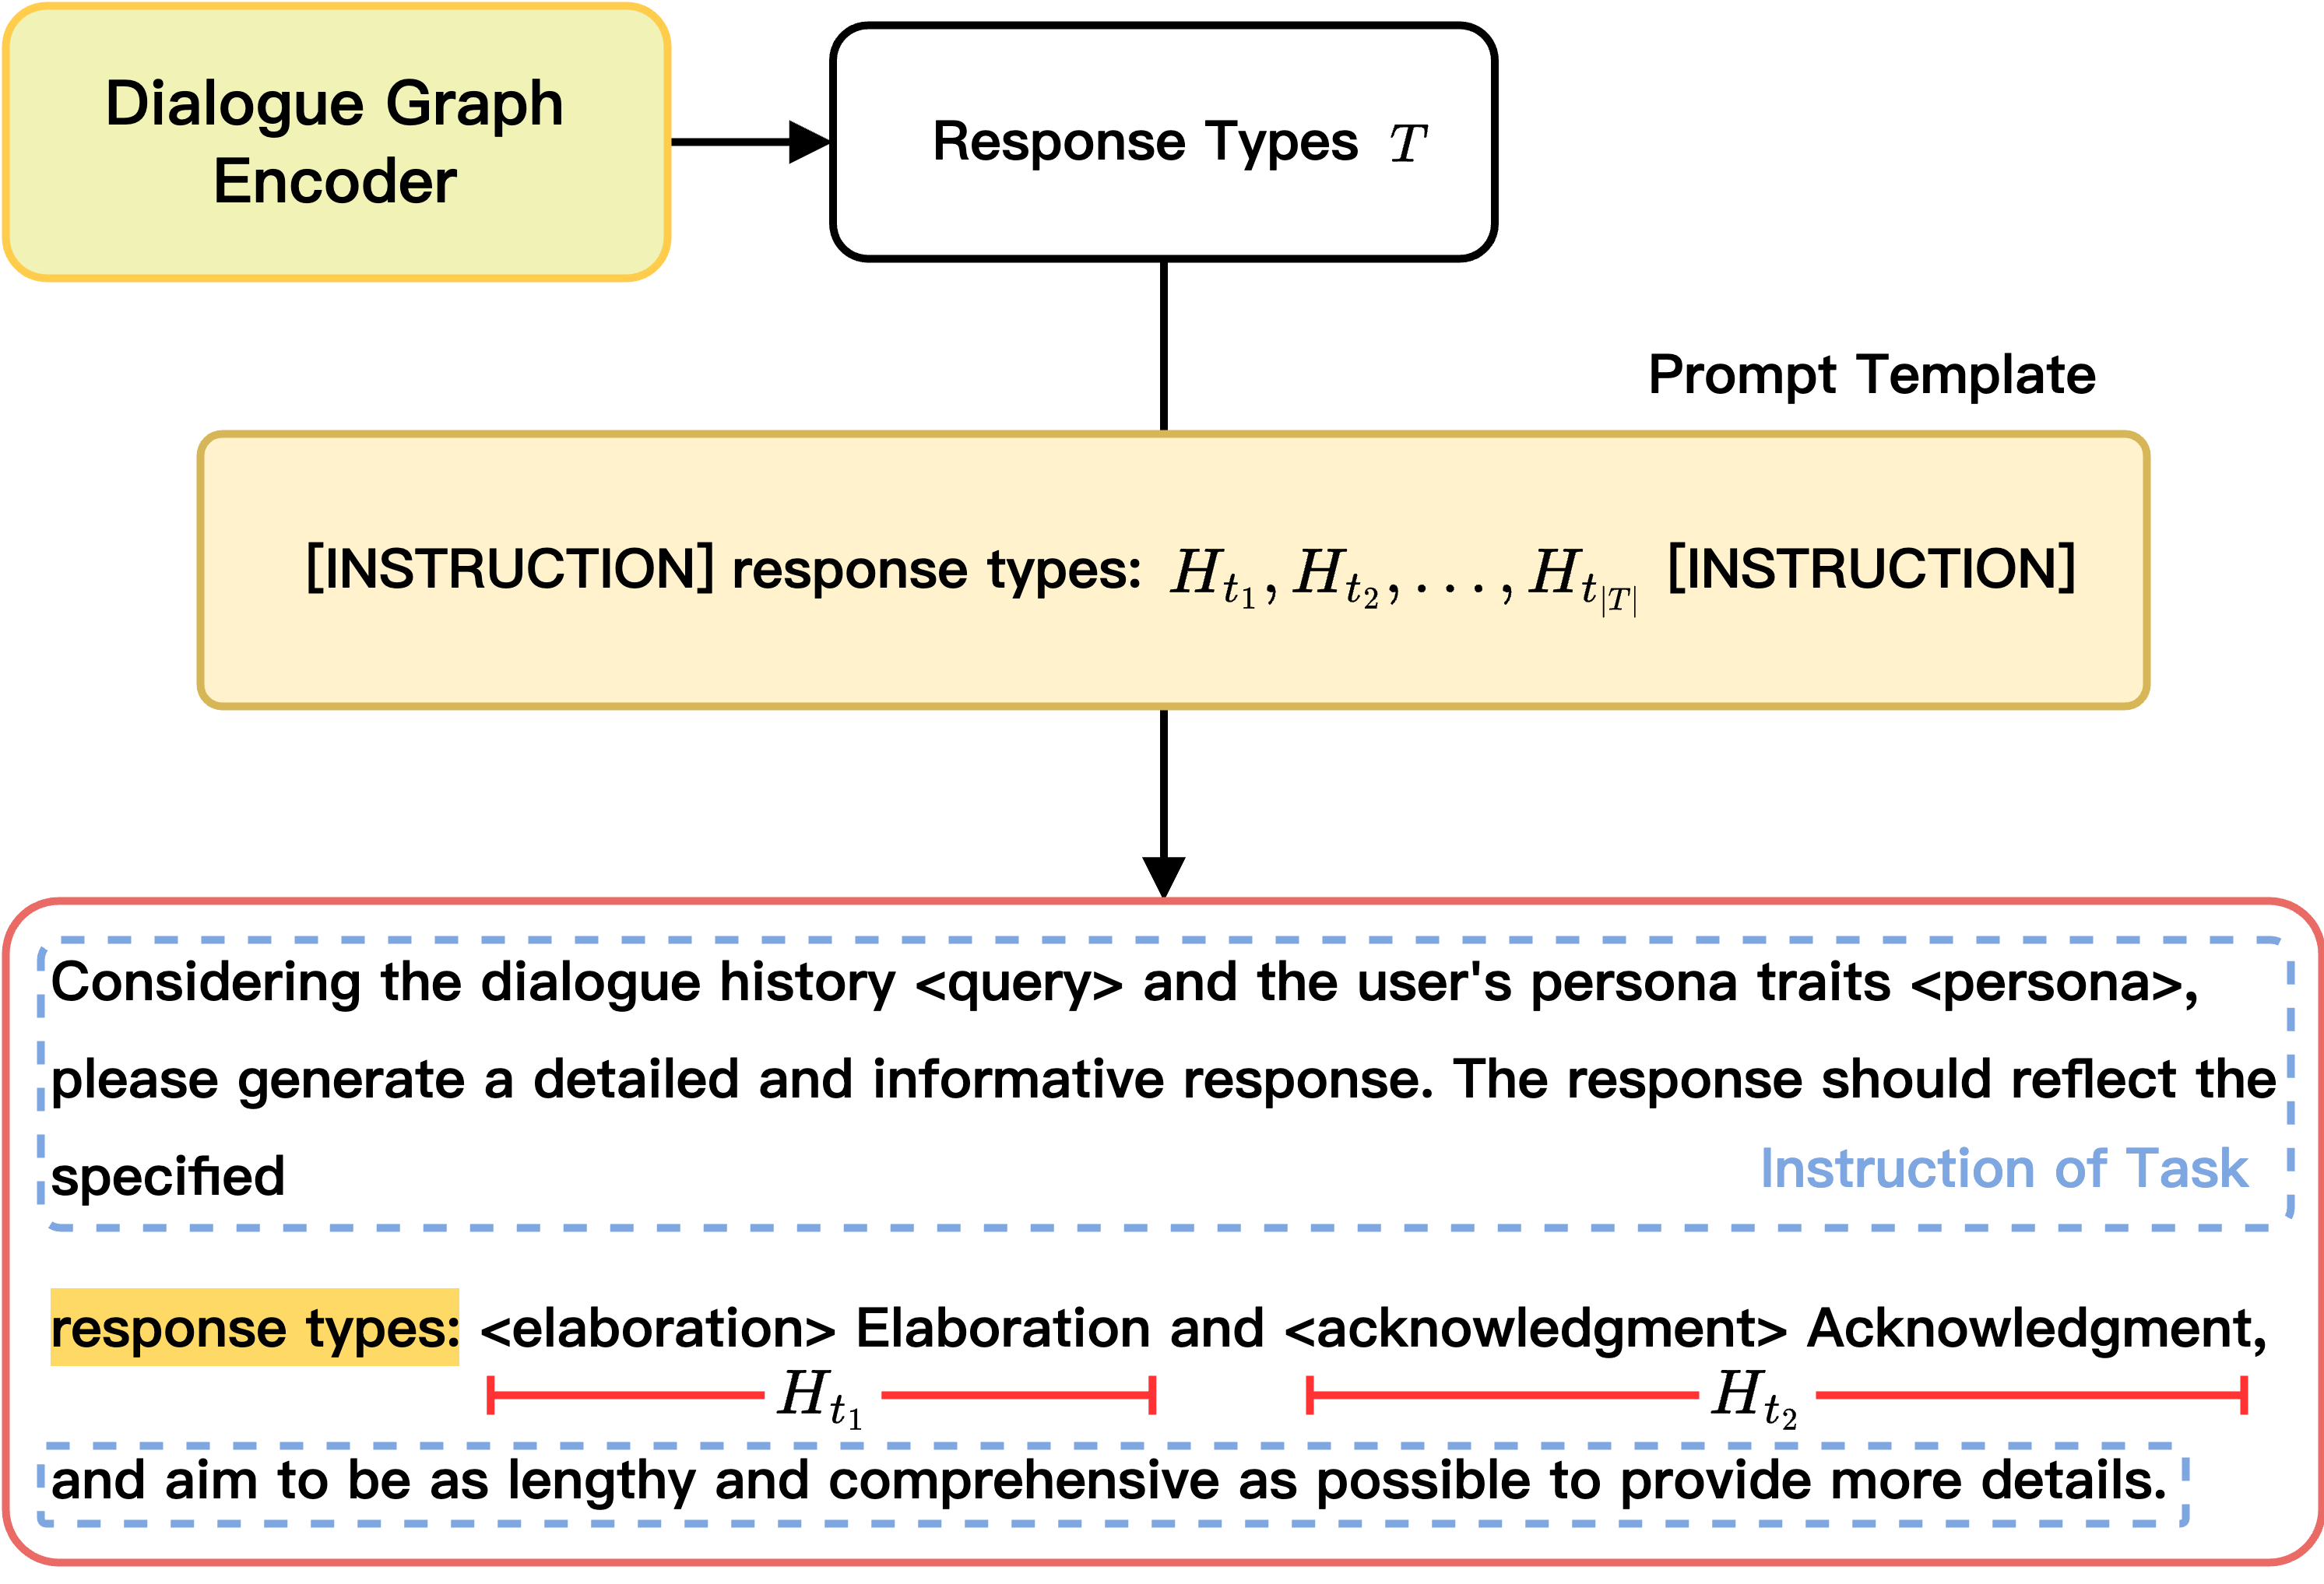
\includegraphics[width=1.00\textwidth]{./context/methodology/images/generator_prompt.png}
    \caption{The Prompt-Tuning pipeline. First, we utilize the dialogue graph encoder to process the context $C$ to predict the $top\text{-}k$ possible next response types $T$. Next, we integrate $T$ into the prompt template. The prompt not only mentions the desired response types but also includes instructions to generate responses, incorporating both persona and context information.}
    \label{fig:generator_prompt}
\end{figure}

Building on the next response type predictions of the Dialogue Graph Encoder, the Prompt Tuning module generates a comprehensive description. This description not only instructs the response generator on how to approach the given task but also guides its generation process by specifying the response types and leveraging both the dialogue context and the persona information.

Therefore, the input sequence for the personalized response generator (BART Decoder) is structured as follows:
\begin{align*}
    E_{\text{Generator}} = [e_{\text{[PROMPT]}}, e_{\text{[BOS]}}, e_{\text{[RSP]}}, e_{\text{1}}^{\text{k}}, e_{\text{2}}^{\text{k}}, ... , e_{\text{|K|-1}}^{\text{k}}, e_{\text{|K|}}^{\text{k}}, e_{\text{[EOS]}}]
\end{align*}

In an encoder-decoder transformer architecture like BART, the decoder references information from the encoder through cross-attention when predicting the next token. To ensure that the generator considers more coherence information while predicting the next token, we apply cross-attention to the dialogue representations generated by the previous two encoders at each transformer block. Thus, during the response generation process, each layer of the decoder performs cross-attention not only on the standard encoder outputs but also on the coherence-aware dialogue representation from the Dialogue Graph Encoder.

Additionally, we propose the Coherence-aware Attention mechanism. We first use learnable embeddings to capture the semantic information of coherence relations. Special tokens representing coherence relations are incorporated into the aforementioned prompt, combining the token embeddings of these special tokens with the coherence embeddings. This mechanism allows the generator to consider the type of response being predicted, such as selecting words that align with an Acknowledgment response type. The coherence-aware attention is visualized in Figure \ref{fig:coherence-aware_attention}. This dual cross-attention mechanism enables the decoder to leverage comprehensive context and persona information, thereby enhancing the coherence and personalization of the generated responses.

\begin{figure}[ht]
    \centering
    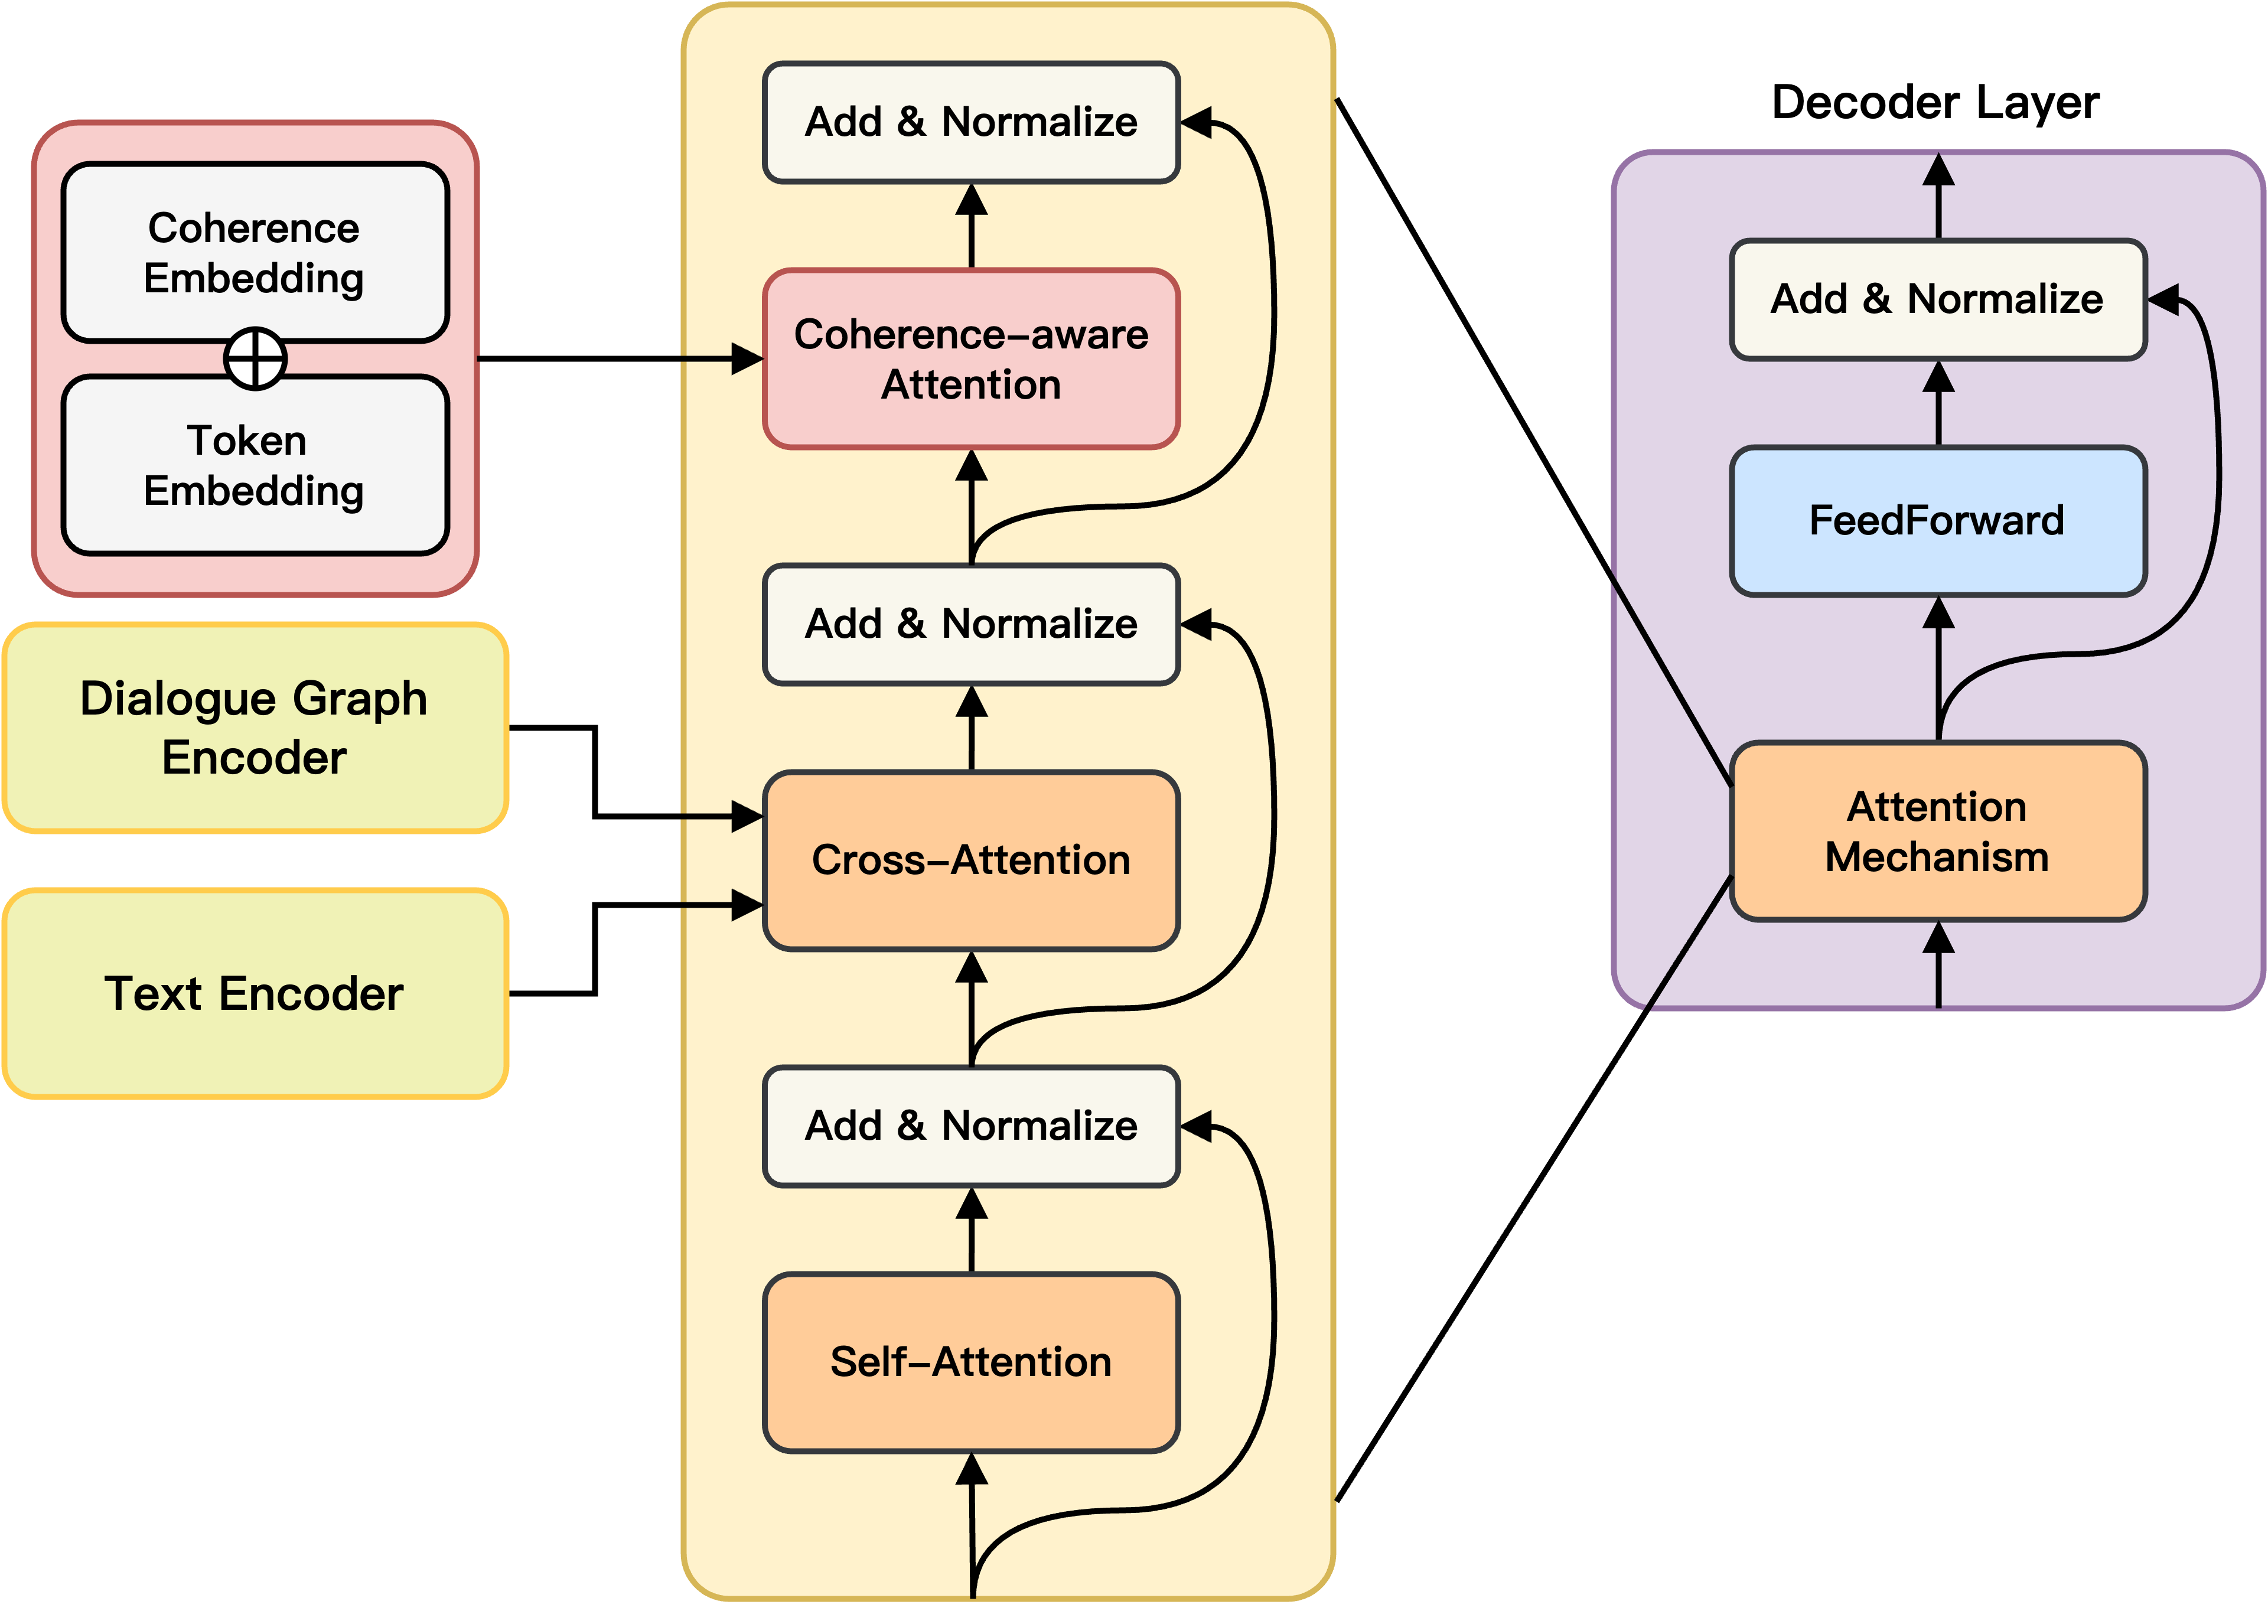
\includegraphics[width=1.00\textwidth]{./context/methodology/images/coherence-aware_attention.png}
    \caption{The visualizations of Coherence-aware Attention. We first compute the cross-attention between the encoder and decoder information. Then, we concatenate the coherence embedding and token embedding of the specified response type with this cross-attention result and perform coherence-aware attention to enrich the discourse information.}
    \label{fig:coherence-aware_attention}
\end{figure}

Finally, to enable the generator to better consider both persona-aware and coherence-aware context information during generation, we are inspired by \cite{huang-etal-2023-paa}. We fuse the decoder hidden states that consider the text encoder information with those that consider the dialogue graph encoder through a Dynamic Weighted Aggregation mechanism. Specifically, we compute a weight $w_{\text{TextEnc}}$ using a sigmoid function over the concatenated hidden states from both encoders (Eq. \ref{eq:dynamic_weighted_aggregation_weight}). Using this weight, we create masked versions of the encoder outputs based on a threshold hyperparameter $\tau$ to control the proportion of persona-aware and coherence-aware information to be considered (Eq. \ref{eq:dynamic_weighted_aggregation_weighting} and \ref{eq:dynamic_weighted_aggregation_mask}). The final output of the generator $O_{\text{Generator}}$ is obtained by adding a residual connection of the original encoder hidden states to the aggregated hidden states, enhancing the coherence and personalization of the generated responses. The detailed formulas are provided in the following equations:

\begin{equation} \label{eq:dynamic_weighted_aggregation_weight}
    w_{\text{TextEnc}} = \sigma(\text{MLP}([H_{\text{TextEnc}} \parallel H_{\text{GraphEnc}}]))
\end{equation}

\begin{equation} \label{eq:dynamic_weighted_aggregation_weighting}
    \begin{aligned}
        O_{\text{TextEnc}} &= w_{\text{TextEnc}} \cdot H_{\text{TextEnc}}, \\
        O_{\text{GraphEnc}} &= (1 - w_{\text{TextEnc}}) \cdot H_{\text{GraphEnc}}
    \end{aligned}
\end{equation}

\begin{equation} \label{eq:dynamic_weighted_aggregation_mask}
    \begin{aligned}
        m_{\text{TextEnc}} &= \mathbb{M}(w_{TextEnc} > \tau), \\
        m_{\text{GraphEnc}} &= \mathbb{M}(1 - w_{TextEnc} > \tau)
    \end{aligned}
\end{equation}

\begin{equation}
    \begin{aligned}
        \hat{O}_{\text{TextEnc}} &= m_{\text{TextEnc}} \odot O_{\text{TextEnc}}, \\
        \hat{O}_{\text{GraphEnc}} &= m_{\text{GraphEnc}} \odot O_{\text{GraphEnc}}, \\
        H_{\text{Enc}} &= \hat{O}_{\text{TextEnc}} + \hat{O}_{\text{GraphEnc}}
    \end{aligned}
\end{equation}

\begin{equation} \label{eq:dynamic_weighted_aggregation_output}
    \begin{aligned}
        H_{\text{residual}} &= H_{\text{TextEnc}} + H_{\text{GraphEnc}}, \\
        O_{\text{Generator}} &= H_{\text{Enc}} + H_{\text{residual}}
    \end{aligned}
\end{equation}

For personalized response generation, we use a language modeling task to compute the probability distribution over the vocabulary for generating the next word given the current context. The language modeling loss, typically implemented as the negative log-likelihood loss, is computed between the predicted probability distribution and the actual next word in the training data. This encourages the model to generate responses that are not only contextually appropriate but also aligned with the persona. The loss function can be formally defined as:

\begin{equation}
    \mathcal{L}_{\text{LM}} = - \sum_{t=1}^{T} \log P(y_t | y_{<t}, O_{\text{Generator}})
\end{equation}

By minimizing this loss function, the model learns to produce fluent and personalized responses that are coherent with the dialogue history and consistent with the persona.

% ------------------------------------------------
\EndChapter
% ------------------------------------------------
